\chapter{Results} \label{chapter_results}

This Chapter is concerned with the presentation of results of the application of
the algorithms at a modular level and the performance of the overall integrated system.

\section{Colour Co-occurrence Histogram}

\section{Mean Shift Tracking}
This section deals with the qualitative analysis of the Mean Shift Tracker
implemented in Section~\ref{implementation_mean_shift_tracker}. The analysis is
broken down into a set of experiments, each of which is based on an image
sequence that exhibits one or more of the challenges to motion tracking outlined
in Section~\ref{literature_review_challenges}. 

The image sequences used are taken from the datasets provided by the VOT2017
challenge \cite{VOT_TPAMI}.

The parameters that are within the control of the User of the MOT System Mean
Shift implementation are.
\begin{itemize}
    \item kernel size 
    \item step threshold, $\epsilon$
    \item number of histogram bins, $m$
\end{itemize}

We subsequently assess the performance of the Mean Shift Tracker implementation
against variations of these three parameters on a diverse set of sequences.
\subsection{Experiment: Effect of bin histogram bin count on Mean Shift Tracker Performance}
\subsubsection{Sequence 1: Fish}
This sequence is one of a several fish, of which a distinctly yellow fish is
tracked. The challenges to motion tracking that arise in this image sequence are the following.
\begin{itemize}
    \item Occlusion (complete)
    \item Scaling 
    \item Ego motion (slight) 
\end{itemize}

The relevant sub-sequences of interest are documented below:

\paragraph{Partial Occlusion}

\begin{figure} \label{fig:mean_shift_partial_occlusion}
    \makebox[\linewidth][c]{
    \begin{tabular}{cccc}
        \subfloat{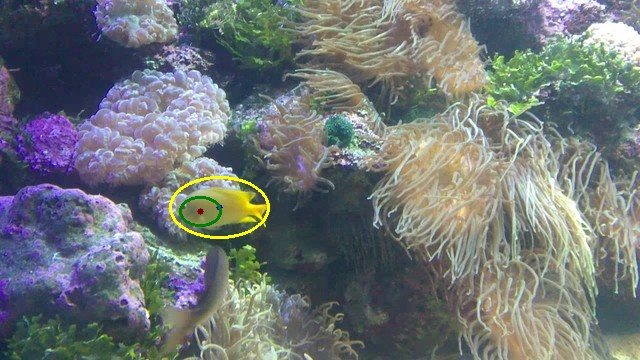
\includegraphics[width = 1.5in]{figures/results/fish3/occlusion/1.jpg}} &
        \subfloat{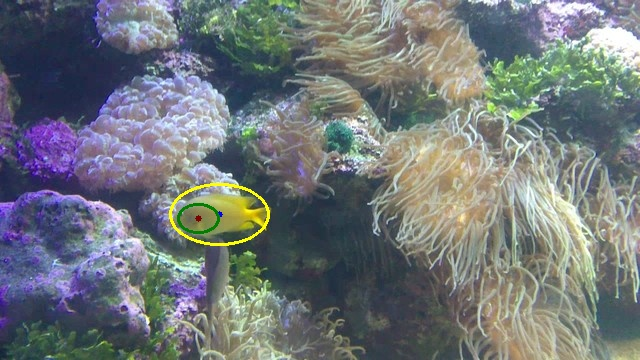
\includegraphics[width = 1.5in]{figures/results/fish3/occlusion/2.jpg}} &
        \subfloat{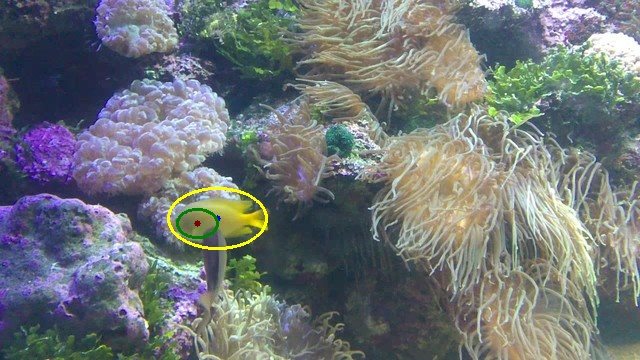
\includegraphics[width = 1.5in]{figures/results/fish3/occlusion/3.jpg}} &
        \subfloat{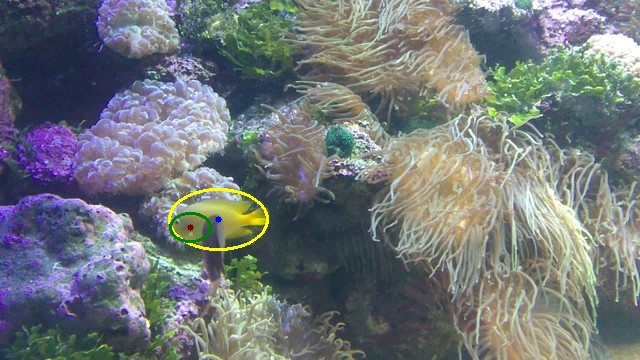
\includegraphics[width = 1.5in]{figures/results/fish3/occlusion/4.jpg}} \\

        \subfloat{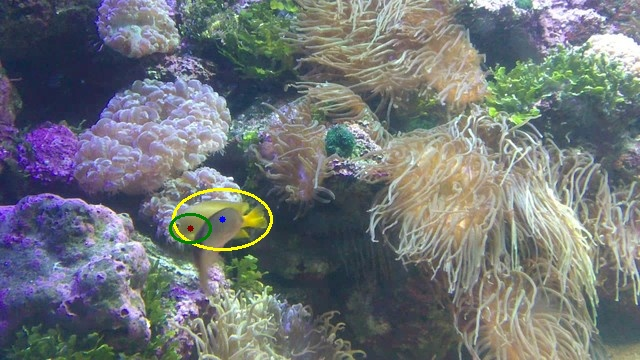
\includegraphics[width = 1.5in]{figures/results/fish3/occlusion/5.jpg}} &
        \subfloat{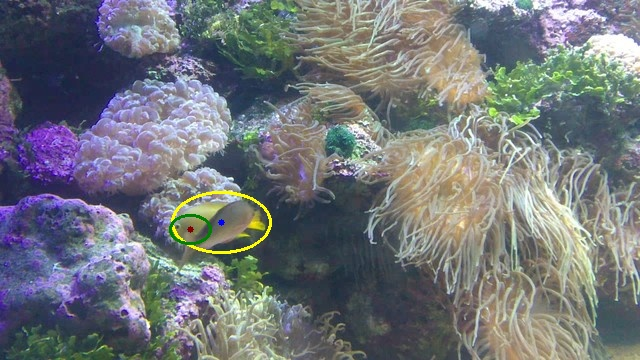
\includegraphics[width = 1.5in]{figures/results/fish3/occlusion/6.jpg}} &
        \subfloat{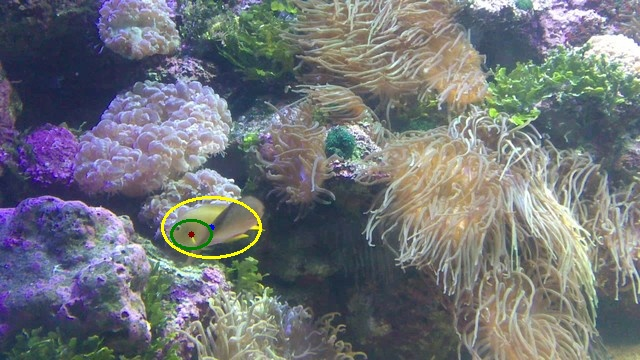
\includegraphics[width = 1.5in]{figures/results/fish3/occlusion/7.jpg}} &
        \subfloat{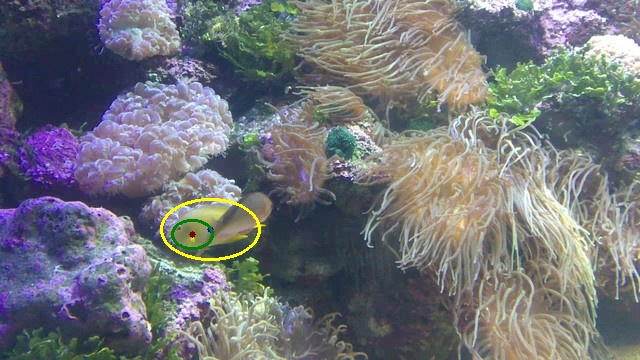
\includegraphics[width = 1.5in]{figures/results/fish3/occlusion/8.jpg}} \\
       
        \subfloat{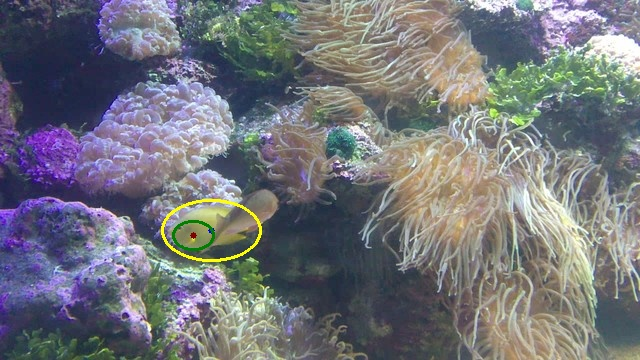
\includegraphics[width = 1.5in]{figures/results/fish3/occlusion/9.jpg}} &
        \subfloat{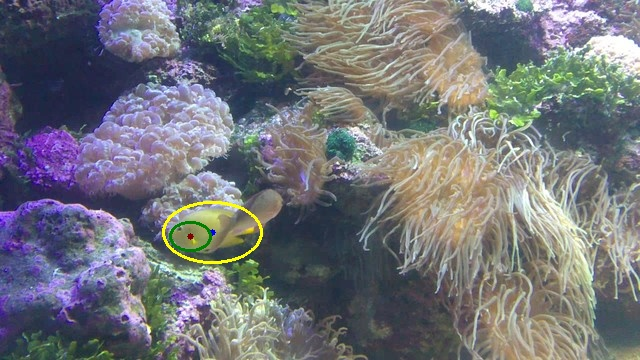
\includegraphics[width = 1.5in]{figures/results/fish3/occlusion/10.jpg}} &
        \subfloat{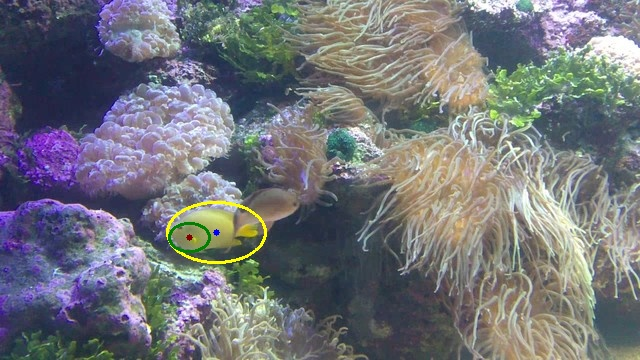
\includegraphics[width = 1.5in]{figures/results/fish3/occlusion/11.jpg}} &
        \subfloat{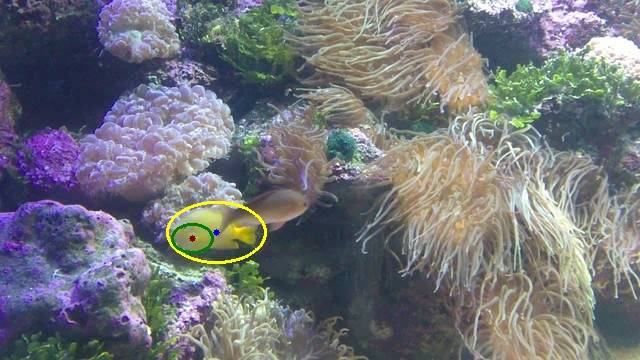
\includegraphics[width = 1.5in]{figures/results/fish3/occlusion/12.jpg}} \\
       
        \subfloat{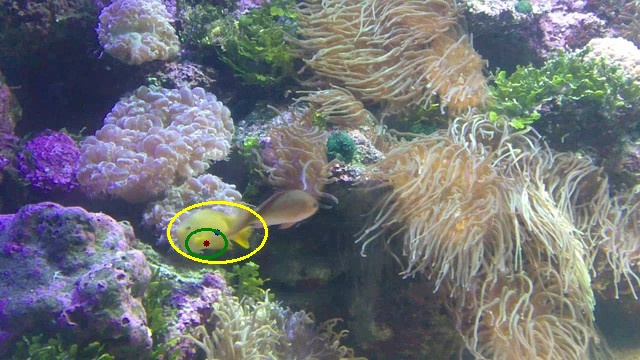
\includegraphics[width = 1.5in]{figures/results/fish3/occlusion/13.jpg}} &
        \subfloat{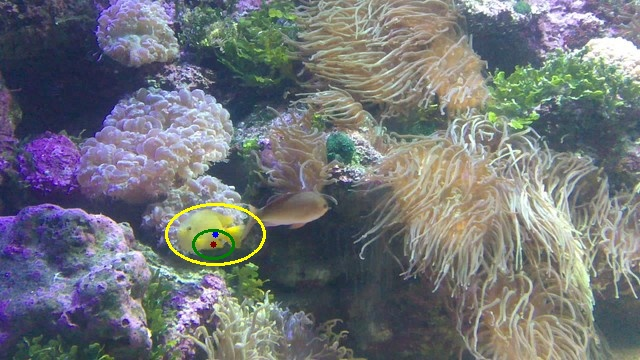
\includegraphics[width = 1.5in]{figures/results/fish3/occlusion/14.jpg}} &
        \subfloat{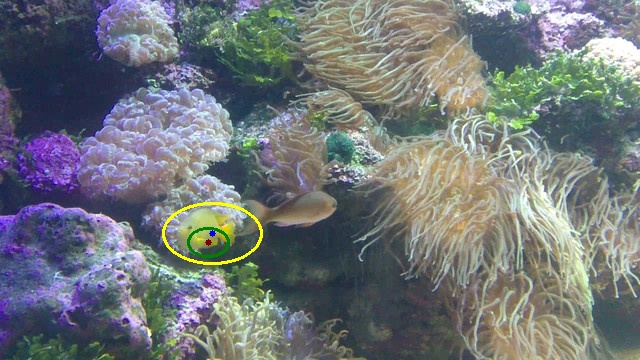
\includegraphics[width = 1.5in]{figures/results/fish3/occlusion/15.jpg}} &
        \subfloat{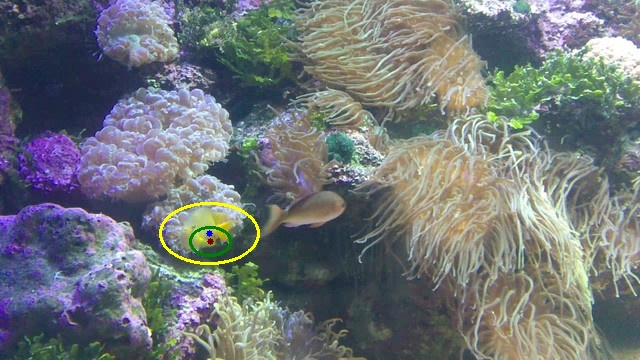
\includegraphics[width = 1.5in]{figures/results/fish3/occlusion/16.jpg}} \\   

        \end{tabular}}
    \caption{Challenge: Partial Occlusion}
\end{figure}

\paragraph{Changing Orientation}

\begin{figure} \label{fig:mean_shift_orientation}
    \makebox[\linewidth][c]{
    \begin{tabular}{cccc}
        \subfloat{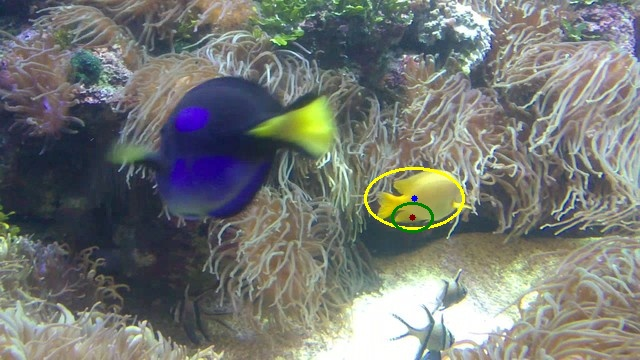
\includegraphics[width = 1.5in]{figures/results/fish3/orientation/1.jpg}} &
        \subfloat{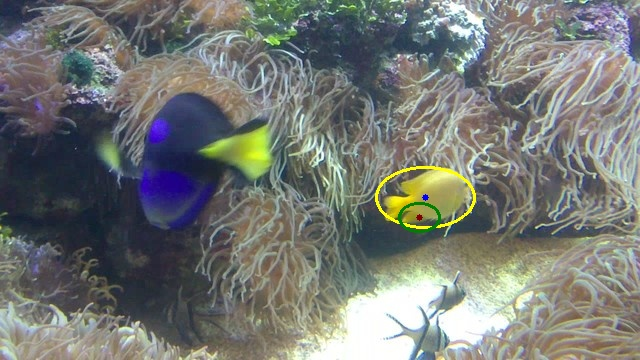
\includegraphics[width = 1.5in]{figures/results/fish3/orientation/2.jpg}} &
        \subfloat{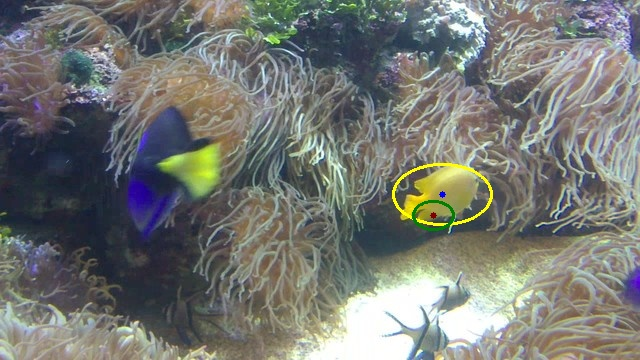
\includegraphics[width = 1.5in]{figures/results/fish3/orientation/3.jpg}} &
        \subfloat{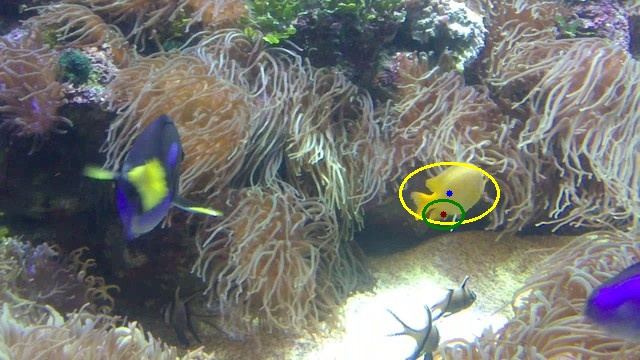
\includegraphics[width = 1.5in]{figures/results/fish3/orientation/4.jpg}} \\

        \subfloat{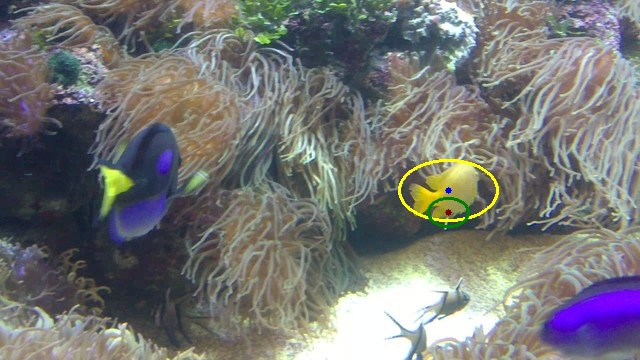
\includegraphics[width = 1.5in]{figures/results/fish3/orientation/5.jpg}} &
        \subfloat{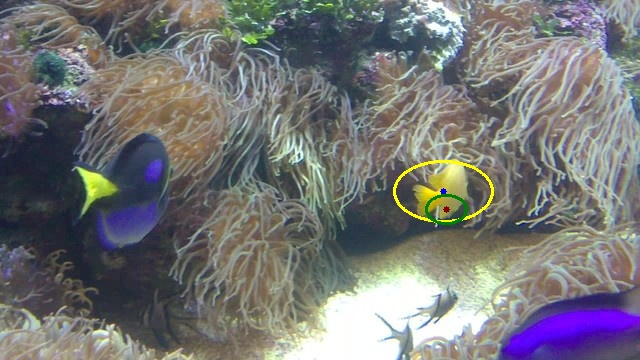
\includegraphics[width = 1.5in]{figures/results/fish3/orientation/6.jpg}} &
        \subfloat{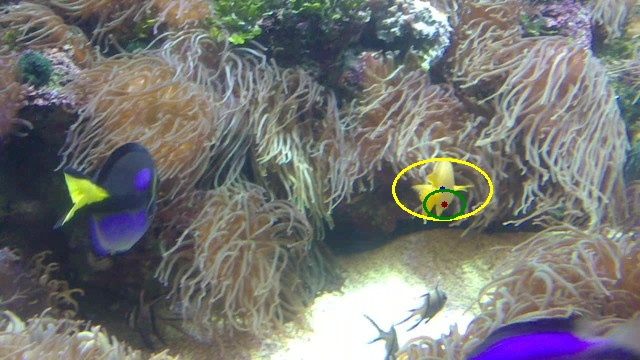
\includegraphics[width = 1.5in]{figures/results/fish3/orientation/7.jpg}} &
        \subfloat{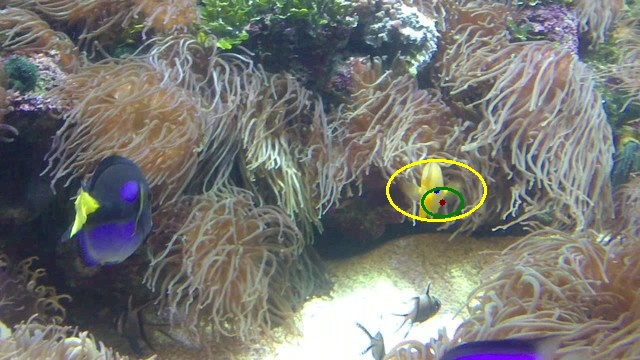
\includegraphics[width = 1.5in]{figures/results/fish3/orientation/8.jpg}} \\
       
        \subfloat{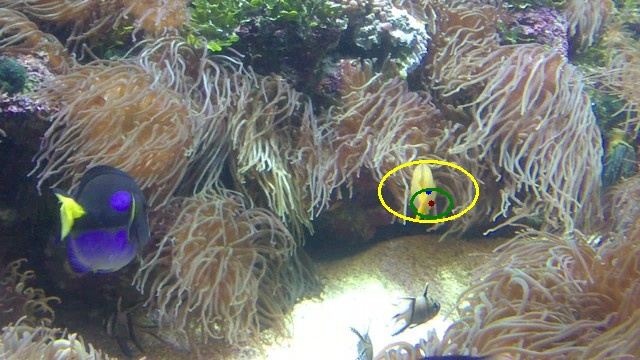
\includegraphics[width = 1.5in]{figures/results/fish3/orientation/9.jpg}} &
        \subfloat{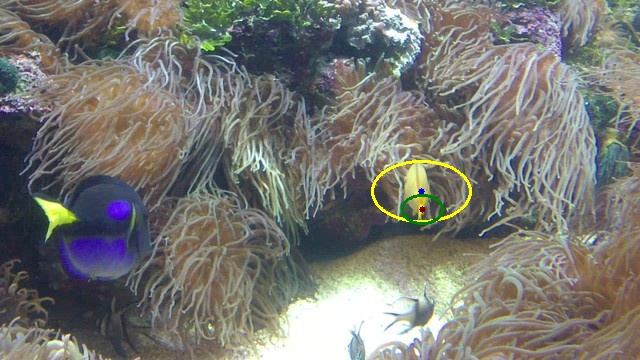
\includegraphics[width = 1.5in]{figures/results/fish3/orientation/10.jpg}} &
        \subfloat{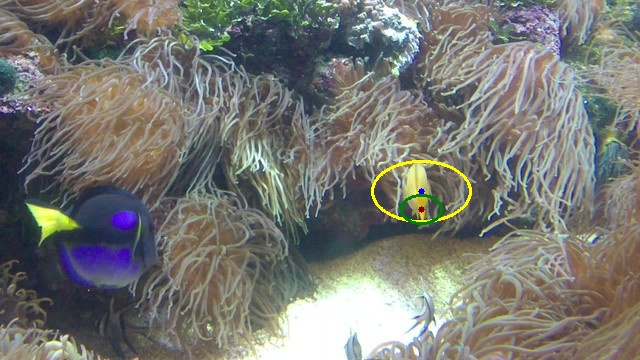
\includegraphics[width = 1.5in]{figures/results/fish3/orientation/11.jpg}} &
        \subfloat{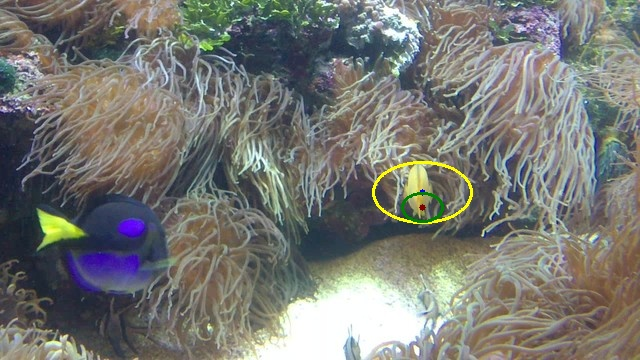
\includegraphics[width = 1.5in]{figures/results/fish3/orientation/12.jpg}} \\
       
        \subfloat{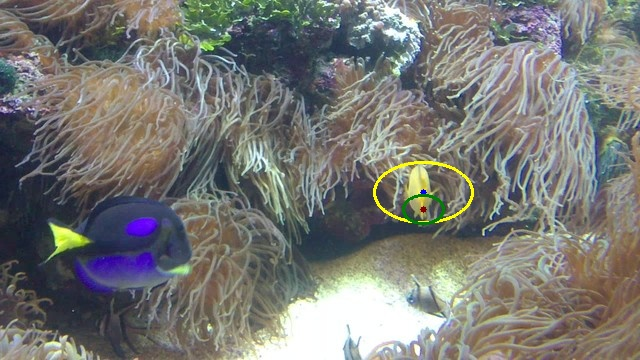
\includegraphics[width = 1.5in]{figures/results/fish3/orientation/13.jpg}} &
        \subfloat{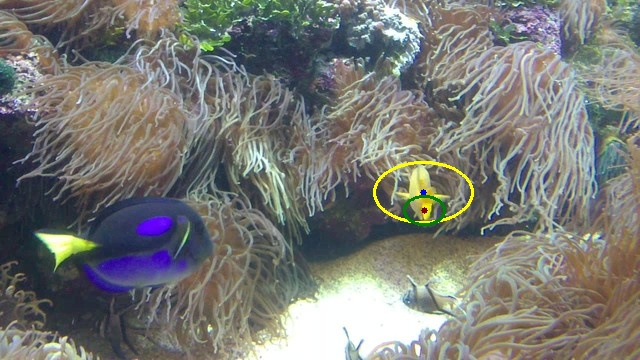
\includegraphics[width = 1.5in]{figures/results/fish3/orientation/14.jpg}} &
        \subfloat{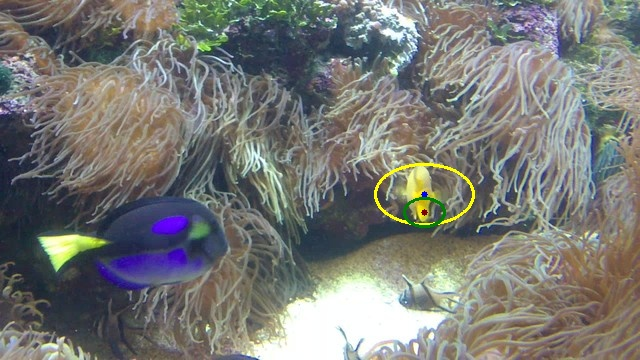
\includegraphics[width = 1.5in]{figures/results/fish3/orientation/15.jpg}} &
        \subfloat{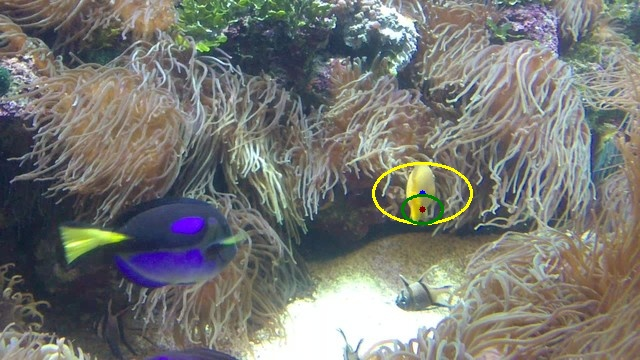
\includegraphics[width = 1.5in]{figures/results/fish3/orientation/16.jpg}} \\   

        \end{tabular}}
    \caption{Challenge: Changing Orientation}
\end{figure}

\subsubsection{Sequence 2: Girl}
This sequence is one of a Girl in a park riding around on a scooter. She is
wearing a distinctive colourful outfit relative to the rest of the moving objects in the
scene, which consist mostly other humans.
The relevant challenges presented in this scene are:
\begin{itemize}
    \item Occlusion (complete)
    \item Scaling 
    \item Ego motion (slight) 
\end{itemize}

\paragraph{Complete Occlusion}
The relevant subsequence exhibiting occlusion ranges from $\mathbf{f}_{97}$ to
$\mathbf{f}_{127}$ and is presented in Figure~\ref{fig:mean_shift_complete_occlusion}.

\begin{figure}    
    \makebox[\linewidth][c]{
    \begin{tabular}{cccc}
        \subfloat{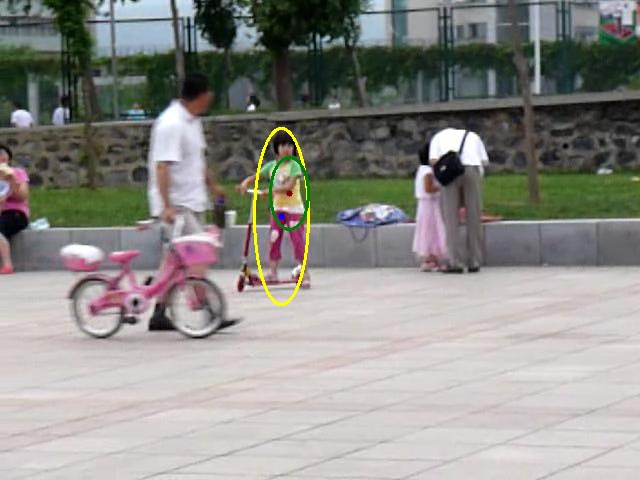
\includegraphics[width = 1.5in]{figures/results/girl/occlusion/1.jpg}} &
        \subfloat{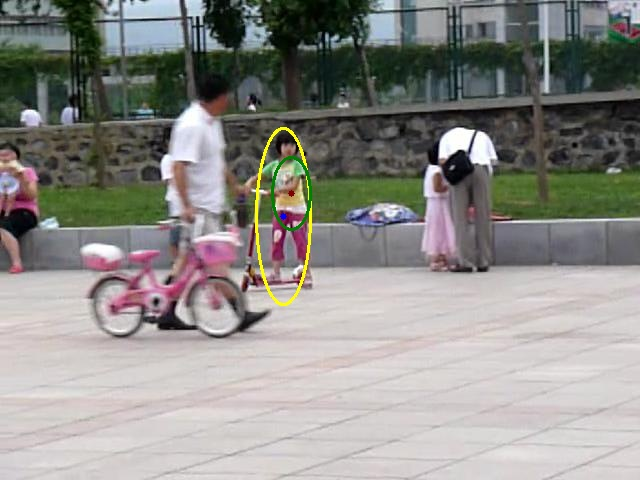
\includegraphics[width = 1.5in]{figures/results/girl/occlusion/2.jpg}} &
        \subfloat{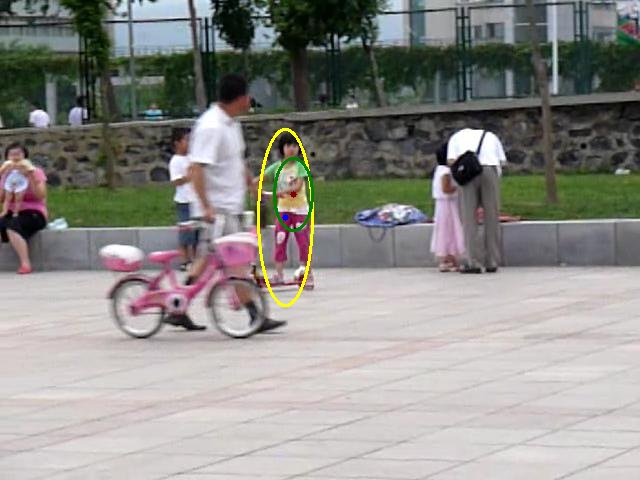
\includegraphics[width = 1.5in]{figures/results/girl/occlusion/3.jpg}} &
        \subfloat{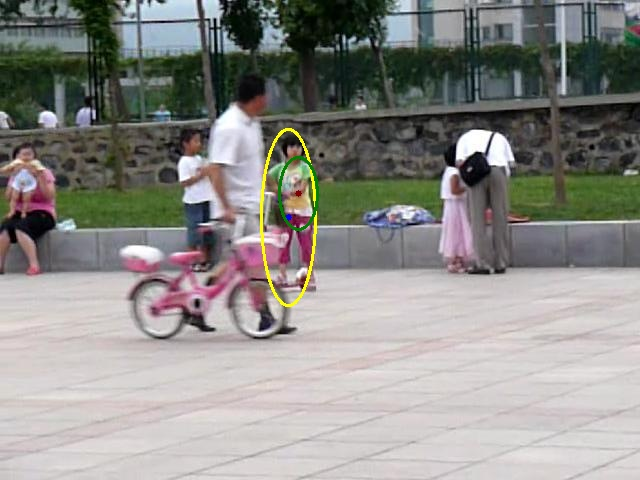
\includegraphics[width = 1.5in]{figures/results/girl/occlusion/4.jpg}} \\

        \subfloat{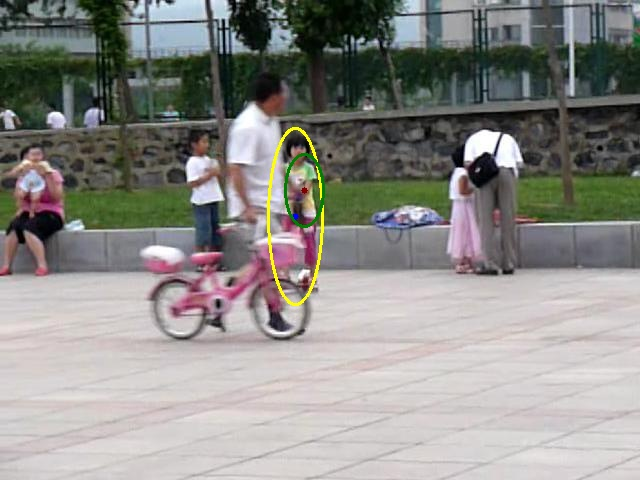
\includegraphics[width = 1.5in]{figures/results/girl/occlusion/5.jpg}} &
        \subfloat{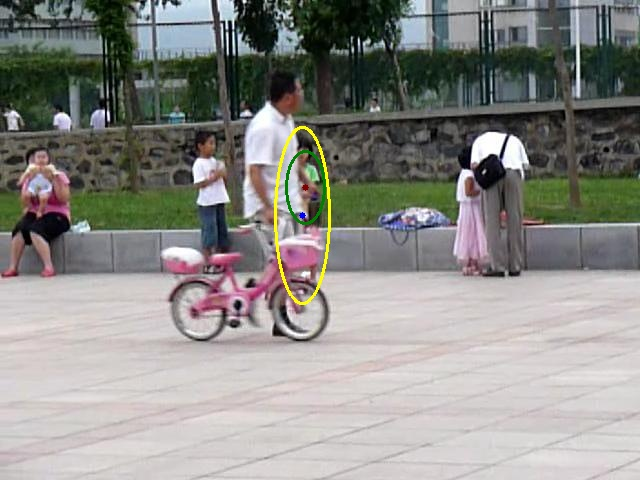
\includegraphics[width = 1.5in]{figures/results/girl/occlusion/6.jpg}} &
        \subfloat{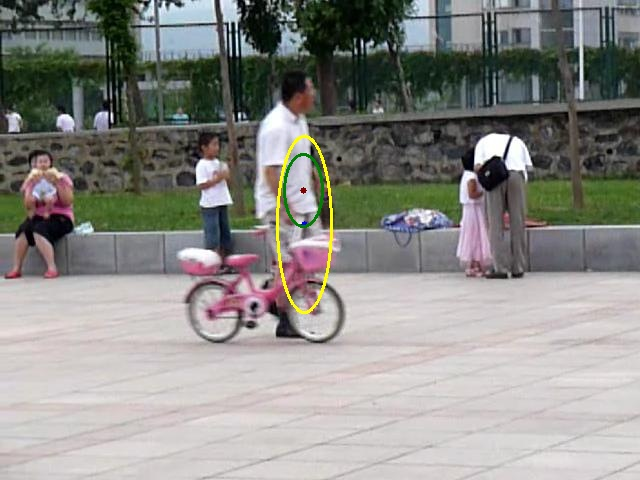
\includegraphics[width = 1.5in]{figures/results/girl/occlusion/7.jpg}} &
        \subfloat{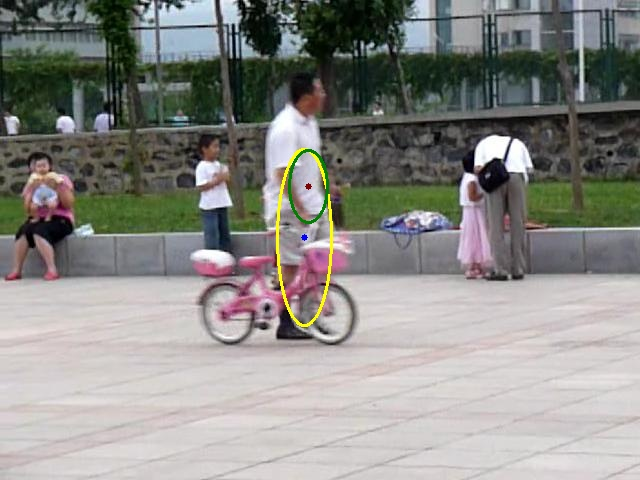
\includegraphics[width = 1.5in]{figures/results/girl/occlusion/8.jpg}} \\
       
        \subfloat{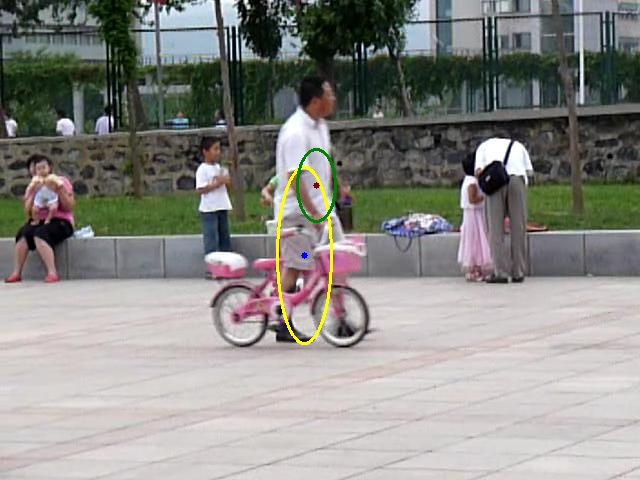
\includegraphics[width = 1.5in]{figures/results/girl/occlusion/9.jpg}} &
        \subfloat{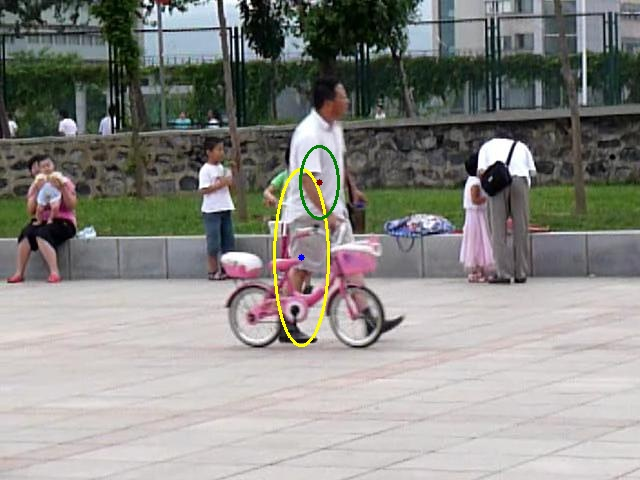
\includegraphics[width = 1.5in]{figures/results/girl/occlusion/10.jpg}} &
        \subfloat{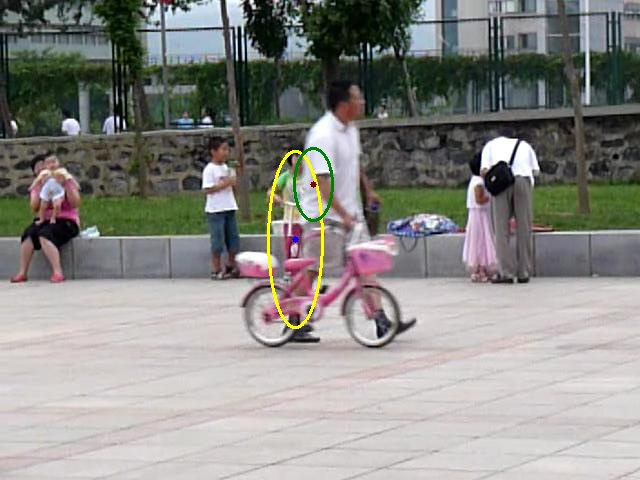
\includegraphics[width = 1.5in]{figures/results/girl/occlusion/11.jpg}} &
        \subfloat{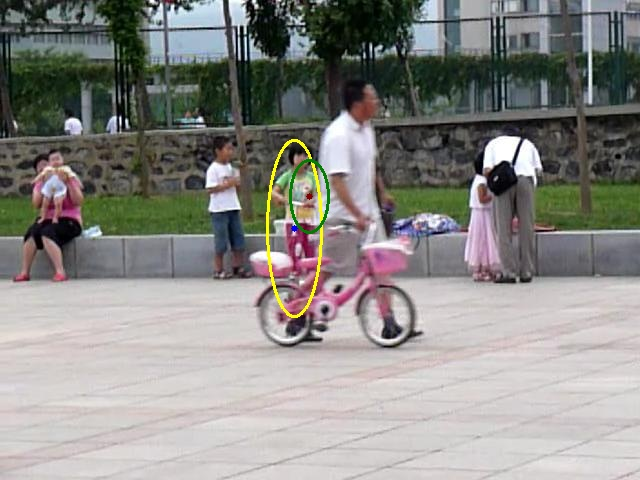
\includegraphics[width = 1.5in]{figures/results/girl/occlusion/12.jpg}} \\
       
        \subfloat{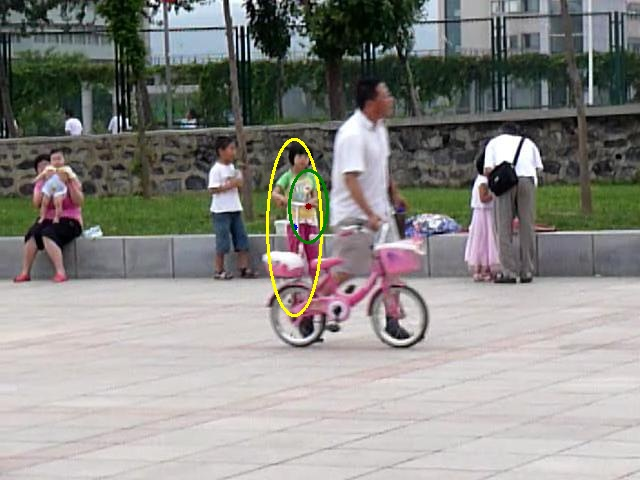
\includegraphics[width = 1.5in]{figures/results/girl/occlusion/13.jpg}} &
        \subfloat{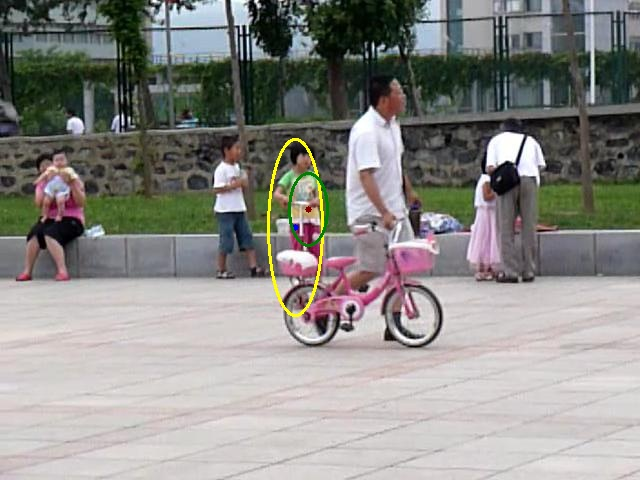
\includegraphics[width = 1.5in]{figures/results/girl/occlusion/14.jpg}} &
        \subfloat{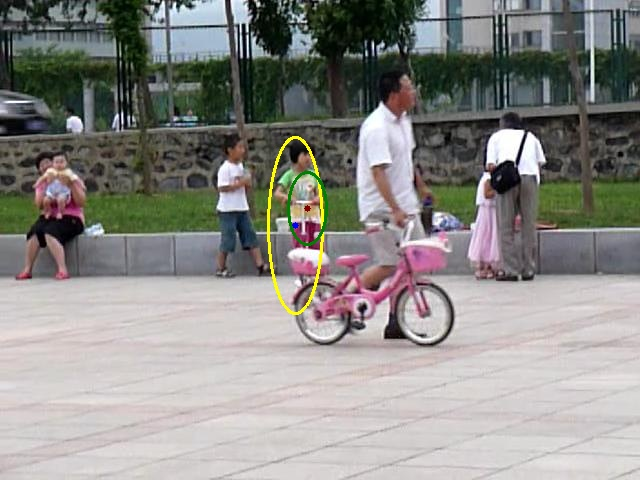
\includegraphics[width = 1.5in]{figures/results/girl/occlusion/15.jpg}} &
        \subfloat{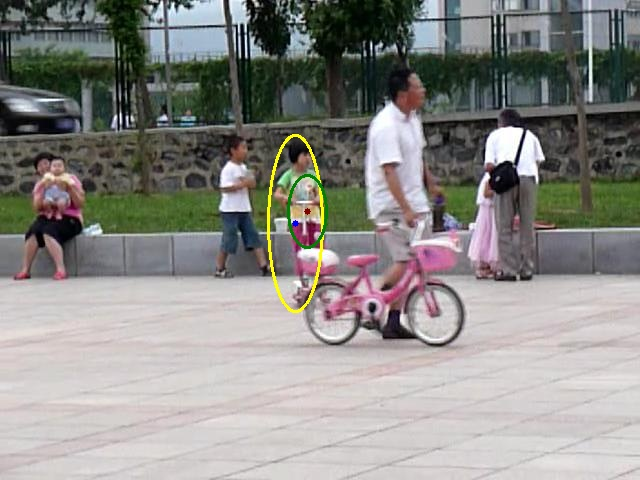
\includegraphics[width = 1.5in]{figures/results/girl/occlusion/16.jpg}} \\   

        \end{tabular}
    }
    \caption{Challenge: Complete Occlusion}
\end{figure}

\paragraph{Scaling}

\begin{figure} \label{fig:mean_shift_girl_scale}
    \makebox[\linewidth][c]{
    \begin{tabular}{cccc}
        \subfloat{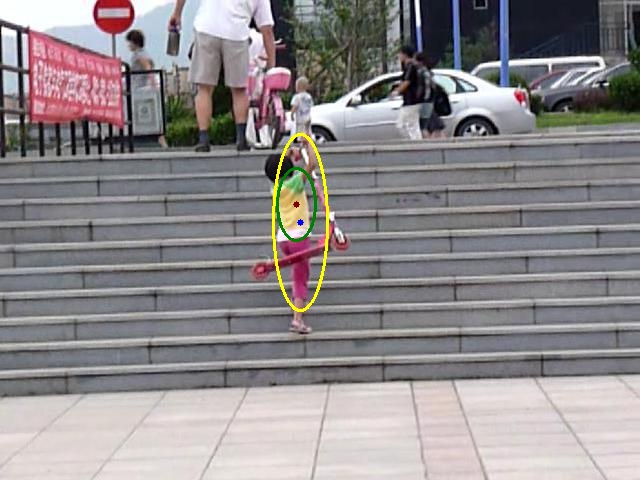
\includegraphics[width = 1.5in]{figures/results/girl/scale/1.jpg}} &
        \subfloat{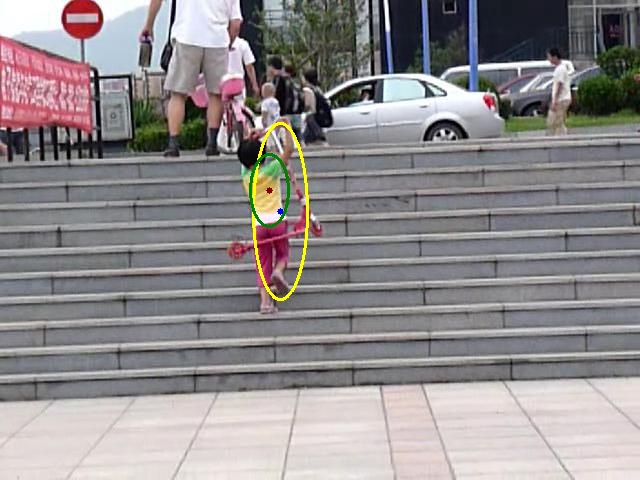
\includegraphics[width = 1.5in]{figures/results/girl/scale/2.jpg}} &
        \subfloat{\includegraphics[width = 1.5in]{figures/results/girl/scale/3.jpg}} &
        \subfloat{\includegraphics[width = 1.5in]{figures/results/girl/scale/4.jpg}} \\

        \subfloat{\includegraphics[width = 1.5in]{figures/results/girl/scale/5.jpg}} &
        \subfloat{\includegraphics[width = 1.5in]{figures/results/girl/scale/6.jpg}} &
        \subfloat{\includegraphics[width = 1.5in]{figures/results/girl/scale/7.jpg}} &
        \subfloat{\includegraphics[width = 1.5in]{figures/results/girl/scale/8.jpg}} \\
       
        \subfloat{\includegraphics[width = 1.5in]{figures/results/girl/scale/9.jpg}} &
        \subfloat{\includegraphics[width = 1.5in]{figures/results/girl/scale/10.jpg}} &
        \subfloat{\includegraphics[width = 1.5in]{figures/results/girl/scale/11.jpg}} &
        \subfloat{\includegraphics[width = 1.5in]{figures/results/girl/scale/12.jpg}} \\
       
        \subfloat{\includegraphics[width = 1.5in]{figures/results/girl/scale/13.jpg}} &
        \subfloat{\includegraphics[width = 1.5in]{figures/results/girl/scale/14.jpg}} &
        \subfloat{\includegraphics[width = 1.5in]{figures/results/girl/scale/15.jpg}} &
        \subfloat{\includegraphics[width = 1.5in]{figures/results/girl/scale/16.jpg}} \\   
    \end{tabular}}
    \caption{Challenge: Scale Change}
\end{figure}


\subsubsection{Sequence 3: Ants}
This image sequence is of multiple ants in motion within a Petri dish.

The challenges presented by this sequence are the following:
\begin{itemize}
    \item Target Speed
    \item Track Overlap
\end{itemize}

\begin{figure} \label{fig:mean_shift_girl_scale}
    \makebox[\linewidth][c]{
    \begin{tabular}{cccc}
        \subfloat{\includegraphics[width = 1.5in]{figures/results/ants/speed/1.jpg}} &
        \subfloat{\includegraphics[width = 1.5in]{figures/results/ants/speed/2.jpg}} &
        \subfloat{\includegraphics[width = 1.5in]{figures/results/ants/speed/3.jpg}} &
        \subfloat{\includegraphics[width = 1.5in]{figures/results/ants/speed/4.jpg}} \\

        \subfloat{\includegraphics[width = 1.5in]{figures/results/ants/speed/5.jpg}} &
        \subfloat{\includegraphics[width = 1.5in]{figures/results/ants/speed/6.jpg}} &
        \subfloat{\includegraphics[width = 1.5in]{figures/results/ants/speed/7.jpg}} &
        \subfloat{\includegraphics[width = 1.5in]{figures/results/ants/speed/8.jpg}} \\
       
        \subfloat{\includegraphics[width = 1.5in]{figures/results/ants/speed/9.jpg}} &
        \subfloat{\includegraphics[width = 1.5in]{figures/results/ants/speed/10.jpg}} &
        \subfloat{\includegraphics[width = 1.5in]{figures/results/ants/speed/11.jpg}} &
        \subfloat{\includegraphics[width = 1.5in]{figures/results/ants/speed/12.jpg}} \\
       
        \subfloat{\includegraphics[width = 1.5in]{figures/results/ants/speed/13.jpg}} &
        \subfloat{\includegraphics[width = 1.5in]{figures/results/ants/speed/14.jpg}} &
        \subfloat{\includegraphics[width = 1.5in]{figures/results/ants/speed/15.jpg}} &
        \subfloat{\includegraphics[width = 1.5in]{figures/results/ants/speed/16.jpg}} \\   
    \end{tabular}}
    \caption{Challenge: Target Speed}
\end{figure}





